\documentclass{article}
\usepackage{graphicx, amsmath, amsthm, tikz, pgfplots, tabularx}
\usepackage{mathrsfs}
\pgfplotsset{compat = newest}
\usepackage[dutch]{babel}
\usepackage[a4paper, total={6in, 8in}]{geometry}

\theoremstyle{definition}
\newtheorem*{Stelling}{Stelling}

\binoppenalty=10000
\relpenalty=10000 

\usetikzlibrary{arrows}

\title{Bewijzen Proefwerk Juni}
\author{Aron Martens}
\date{March 2025}

\begin{document}

\maketitle

\section{Bepaalde integraal p.16}
Stel dat $f$ een positieve, continue functie is in $\left[a,b\right]$. We zoeken de oppervlakte van het gebied tussen $f$ en de x-as.
\begin{enumerate}
  \item Verdeel $\left[a,b\right]$ in $n$ intervallen met breedte $\Delta{x}=\frac{b-a}{n}.$
  \item Bereken in elk interval het minimum $m_i$ en maximum $M_i$. Aangezien $f$ continu is, zijn deze altijd te vinden. (Stelling van Weierstrass).
  \item Bereken de ondersom en de bovensom: $$s_n=\sum_{i=1}^{n}m_i\cdot \Delta{x}\quad\quad \text{en} \quad\quad S_n=\sum_{i=1}^{n}M_i\cdot \Delta{x}$$
  \item We definiëren de bepaalde integraal als $$\lim_{n\to \infty }s_n = \lim_{n\to + \infty}S_n=\int_a^bf(x)\,dx$$
\end{enumerate}

\subsection{Opmerking Riemannsom p.16}
Bernhard Rimemann toonde aan dat je het minimum of maximum niet nodig hebt. Een willekeurige functiewaarde $f\left(x_i\right)$ volstaat.
\begin{proof}
  \begin{align*}
  m_i \leq &f\left(x_i\right) \leq M_i\\
           &\Downarrow \\
  m_i \cdot \Delta{x} \leq &f\left(x_i\right) \cdot \Delta{x}\leq M_i\cdot \Delta{x}\\
                           &\Downarrow \\
  \sum_{i=1}^{n}m_i\cdot \Delta x \leq \sum_{i=1}^{n} &f\left(x_i\right)\cdot \Delta x \leq \sum_{i=1}^{n} M_i \cdot \Delta{x}\\
                                                      &\Downarrow \\
  s_n \leq \sum_{i=1}^{n} &f\left(x_i\right) \cdot \Delta x \leq S_n\\
  \end{align*}
  Omdat $\displaystyle\lim_{n\to \infty}s_n = \displaystyle\lim_{n\to + \infty}S_n = \displaystyle\int_{a}^{b}f(x)\,dx,$ volgt uit de insluitstelling dat
  $$\lim_{n\to + \infty}\sum_{i=1}^{n}f(x_i)\cdot \Delta x = \displaystyle\int_{a}^{b}f(x)\,dx$$.
\end{proof}

\section{Integraal van $x^0 = 1$ p.19}
\begin{align*}
  \displaystyle\int_{a}^{b} x^0 \, dx &= \lim_{n\to + \infty} \frac{b-a}{n}\cdot\sum_{i=1}^{n}1\\
                                     &=\lim{n\to + \infty}\frac{b-a}{n}\cdot n\\
                                     &=b-a
\end{align*}
\section{Integraal van $x$ p.20}
We verdelen $[a,b]$ in $n$ deelintervallen met breedte $\Delta x = \frac{b-a}{n}.$ Als $x_i$ nemen we de linkergrens van elk interval. 
\begin{center}
  \begin{tabularx}{\textwidth}{| >{\centering\arraybackslash}X | >{\centering\arraybackslash}X | >{\centering\arraybackslash}X|}
    \hline
    INTERVAL & $x_i$ & $f\left(x_i\right) = x_i$\\
    \hline
    \hline
    $\left[a, a+\Delta x\right]$ & $a$ & $a$\\
   \hline
    $\left[a + \Delta x, a+2\Delta x\right]$ & $a+\Delta x$ & $a+\Delta x$\\
    \hline
    $\left[a + 2\Delta x, a+3\Delta x\right]$ & $a+2\Delta x$ & $a+2\Delta x$\\
    \hline
    $\cdots$ &$\cdots$ &$\cdots$\\
    \hline
    $\left[a + \left(n-1\right)\Delta x, b\right]$ & $a+\left(n-1\right)\Delta x$ & $a+\left(n-1\right)\Delta x$\\
    \hline
  \end{tabularx}
\end{center}


\begin{align*}
  \displaystyle\int_{a}^{b}x\,dx &=\lim_{n\to + \infty} \frac{b-a}{n}\cdot\left[a+\left(a+\Delta x\right) + \left(a+2\Delta x\right) + \cdots + \left(a+\left(n-1\right)\Delta x\right)\right]\\
                                 &=\lim_{n\to + \infty}\frac{b-a}{n}\cdot\frac{n\cdot\left(a+a+\left(n-1\right)\Delta x\right)}{2} &\left(s=\frac{u_1+u_n}{2}\cdot n\right)\\
                                 &=\lim_{\Delta x\to 0}\frac{\left(b-a\right)\cdot\left(a+b-\Delta x\right)}{2}\\
                                 &=\frac{b^2-a^2}{2}
\end{align*}

\section{Integraal van $x^2$ p.21}
\subsection{Over het interval $\left[0,b\right]$ met $b>0$}
We verdelen $\left[0,b\right]$ in $n$ deelintervallen met breedte $\Delta x = \frac{b}{n}.$ Als $x_i$ nemen we de rechtergrens van elk interval.
\begin{center}
  \begin{tabularx}{\textwidth}{| >{\centering\arraybackslash}X | >{\centering\arraybackslash}X | >{\centering\arraybackslash}X|}
    \hline
    INTERVAL & $x_i$ & $f\left(x_i\right) = x_i^2$\\
    \hline
    \hline
    $\left[0, \Delta x\right]$ & $\Delta x$ & $1\left(\Delta x\right)^2$\\
   \hline
    $\left[\Delta x, 2\Delta x\right]$ & $2\Delta x$ & $4\left(\Delta x\right)^2$\\
    \hline
    $\left[2\Delta x, 3\Delta x\right]$ & $3\Delta x$ & $9\left(\Delta x\right)^2$\\
    \hline
    $\cdots$ &$\cdots$ &$\cdots$\\
    \hline
    $\left[\left(n-1\right)\Delta x, b\right]$ & $n\Delta x = b$ & $n^2\left(\Delta x\right)^2$\\
    \hline
  \end{tabularx}
\end{center}

\begin{align*}
  \displaystyle\int_{0}^{b}x^2\, dx &= \lim_{n\to + \infty}\frac{b}{n}\left(\left(1+4+9+\cdots+n^2\right)\cdot\left(\Delta x\right)^2\right)\\
                                    &=\lim_{n\to + \infty}\frac{b}{n}\frac{n\cdot\left(n+1\right)\left(2n+1\right)}{6}\cdot \frac{b^2}{n^2}\\
                                    &=\frac{b^3}{6}\lim_{n\to + \infty}\frac{2n^3}{n^3}\\
                                    &= \frac{b^3}{3}
\end{align*}
\subsection{Over het interval $\left[a,b\right]$ met $0<a<b$}
\begin{align*}
  \displaystyle\int_{a}^{b}x^2\,dx &= \displaystyle\int_{0}^{b}x^2\, dx - \displaystyle\int_{0}^{a}x^2 \, dx\\
                                   &= \frac{b^3}{3} - \frac{a^3}{3}
\end{align*}
\subsection{Over het interval $\left[a,b\right]$ met $a<0\leq b$}
\begin{align*}
  \displaystyle\int_{a}^{b}x^2\,dx&=\displaystyle\int_{a}^{0}x^2\,dx + \displaystyle\int_{0}^{b}x^2\,dx\\
                                  &=\displaystyle\int_{0}^{-a}x^2\,dx + \displaystyle\int_{0}^{b}x^2\,dx\\
                                  &=-\frac{a^3}{3} + \frac{b^3}{3}
\end{align*}
\subsection{Over het interval $\left[a,b\right]$ met $a<b\leq 0$}
\begin{align*}  
\displaystyle\int_{a}^{b}x^2\, dx &= \displaystyle\int_{-b}^{-a}x^2\,dx\\
                                  &=\frac{\left(-a^3\right)}{3}-\frac{\left(-b^3\right)}{3}\\
                                  &=-\frac{a^3}{3}+\frac{b^3}{3}
\end{align*}
\section{Middelwaardestelling van de integraalrekening p.31}
\begin{Stelling}
  Als $f$ continu is in $\left[a,b\right]$, dan bestaat er een $c \in \left[a, b\right]: \displaystyle\int_{a}^{b}f\left(x\right)\,dx = \left(b-a\right)\cdot f\left(c\right)$
\end{Stelling}

\begin{proof}
  We hebben 3 gevallen:
  \begin{enumerate}
    \item $\boxed{a<b}$\\
      We verdelen $\left[a,b\right]$ in $n$ intervallen met breedte $\Delta x = \frac{b-a}{n}$.\\
      \begin{align*}
        \text{Dan geldt:}\qquad m\leq &f\left(x_i\right) \leq M\\
                          &\Downarrow\\
        m \cdot \Delta x\leq &f\left(x_i\right)\cdot \Delta x \leq M\cdot \Delta x\\ 
                          &\Downarrow\\
        n\cdot m \cdot \Delta x\leq \sum_{i=1}^{n}&f\left(x_i\right)\cdot \Delta x \leq n\cdot M\cdot \Delta x\\
                          &\Downarrow\\
        m\cdot \left(b-a\right)\leq \lim_{n\to + \infty}\sum_{i=1}^{n}f\left(x_i\right)\cdot \Delta x &=\displaystyle\int_{a}^{b}f\left(x\right)\,dx\leq M\cdot \left(b-a\right)\\
                          &\Downarrow\\
        m\leq\frac{1}{b-a}&\displaystyle\int_{a}^{b}f\left(x\right)\,dx\leq M
      \end{align*}
      Volgens de stelling van Weierstrass en de tussenwaardestelling bestaat er in $\left[a,b\right]$ minstens één $c$ zodat
      $$f\left(c\right)=\frac{1}{b-a}\displaystyle\int_{a}^{b}f\left(x\right)\,dx, \quad \text{dus} \quad  \displaystyle\int_{a}^{b}f\left(x\right)\,dx=\left(b-a\right)\cdot f\left(c\right)$$
    \item $\boxed{a=b}$\\
      Dan is $\displaystyle\int_{a}^{b}f\left(x\right)\, dx= 0 = \left(b-a\right)\cdot f\left(c\right)$
    \item $\boxed{a>b}$\\
      \begin{align*}
        \text{Uit \textbf{1} volgt dan: } \exists c\in \left[a,b\right]: \displaystyle\int_{a}^{b}f\left(x\right)\,dx &= \left(a-b\right)\cdot f\left(c\right)\\
                                                                                                                       &\Downarrow\\
         \exists c\in \left[a,b\right]: -\displaystyle\int_{b}^{a}f\left(x\right)\,dx &= \left(a-b\right)\cdot f\left(c\right)\\
                                                                                                                       &\Downarrow\\
         \exists c\in \left[a,b\right]: \displaystyle\int_{b}^{a}f\left(x\right)\,dx &= \left(b-a\right)\cdot f\left(c\right)\\
      \end{align*}
  \end{enumerate}
\end{proof}

\section{Hoofdstelling van de integraalrekening}
\begin{Stelling}
  Als $f$ continu is in $\left[a,b\right]$, dan geldt in $\left[a,b\right]$: $I_a^{'} \left(x\right) = f\left(x\right)$.
\end{Stelling}
\begin{proof}
  We bewijzen dat $\forall x \in \left[a,b\right]: \displaystyle\lim_{\Delta x \to 0} \dfrac{I_a\left(x+\Delta x\right) - I_a\left(x\right)}{\Delta x} = f\left(x\right)$
\begin{align*}
  \lim_{\Delta x \to 0} \dfrac{I_a\left(x+\Delta x\right) - I_a\left(x\right)}{\Delta x} &= \frac{\displaystyle\int_{a}^{x+\Delta x}f\left(t\right)\, dt - \displaystyle\int_{a}^{x}f\left(t\right)\, dt}{\Delta x}\\
                                                                                         &= \frac{\displaystyle\int_{a}^{x+\Delta x}f\left(t\right)\, dt + \displaystyle\int_{x}^{a}\left(t\right)\, dt}{\Delta x}\\
                                                                                         &= \frac{\displaystyle\int_{x}^{x+\Delta x}f\left(t\right)\, dt}{\Delta x}\\
                                                                                         &=\frac{\left(x+\Delta x -x\right)\cdot f\left(c\right)}{\Delta x}\\
                                                                                         &=f\left(c\right) \qquad \text{met } c\in \left[x, x+\Delta x\right],\\
                                                                                         \intertext{dus}
  \displaystyle\lim_{\Delta x \to 0} \dfrac{I_a\left(x+\Delta x\right) - I_a\left(x\right)}{\Delta x} &= \lim_{\Delta x \to 0} f\left(c\right)\\
                                                                                                      &=f\left(x\right)
\end{align*}
\end{proof}


\section{Oppervlakte van een cirkel p.119}
\begin{Stelling}
    De oppervlakte van een cirkel met straal $r$ is $\pi r^2$
\end{Stelling}

\begin{proof}
De vergelijking van een cirkel is $$x^2+y^2=r^2.$$
Dan is de vergelijking in het eerste kwadrant:
$$y=\sqrt{r^2-x^2}.$$
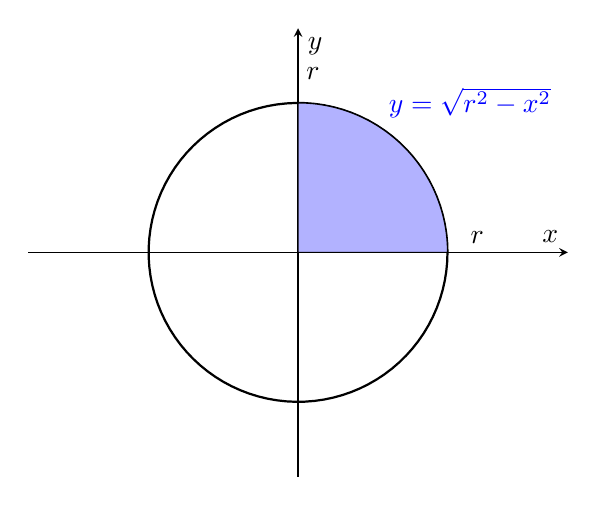
\begin{tikzpicture}

\begin{axis}[
axis equal,
xlabel=$x$, 
ylabel=$y$,
xmin = -1.5, xmax = 1.5, ymin = -1.5, ymax=1.5,
grid = none,
axis lines = center,
xtick={0},
ytick={0}
]

        \addplot [domain=0:360, samples=100, thick] ({cos(x)}, {sin(x)});
        \addplot [domain=0:90, samples=50, fill=blue!30] ({cos(x)}, {sin(x)}) -- (axis cs:0,0) -- cycle;
        \node at (axis cs:0.1,1.2) {$r$};
        \node at (axis cs:1.2,0.1) {$r$};
        
        \node at (axis cs:1.15,1){\textcolor{blue}{$y=\sqrt{r^2-x^2}$}};
        

\end{axis}
\end{tikzpicture}   
De oppervlakte is dus
$$A=4\cdot \int_0^r\sqrt{r^2-x^2}\, dx$$
Stel $x=r\sin t$ en $t\in\left[-\frac{\pi}{2},\frac{\pi}{2}\right]$, dan is $dx =r\cos t\, dt$. 
\\ Dan is $$\sqrt{r^2-x^2}\,dx = \sqrt{r^2-r^2\sin^2t}\, dx=r\sqrt{\cos^2t}\cdot r\cos t\,dt = r^2\cos^2t\,dt.$$
Als $x=0$, dan is $r\sin t = 0$ of $t=0$.\\
Als $x=r$, dan is $r\sin t = r$ of $t=\frac{\pi}{2}$.\\
Dus $$A = 4\cdot\int_0^r \sqrt{r^2-x^2}\, dx =4r^2\int_0^\frac{\pi}{2}\cos^2t\,dt = 4r^2\int_0^\frac{\pi}{2} \frac{1+\cos2t}{2}\,dt = 2r^2\left[t + \frac{\sin2t}{2}\right]_0^\frac{\pi}{2}$$ $$=\\ 2r^2\cdot\frac{\pi}{2} = \pi r^2.$$


\end{proof}\newpage
\section{Oppervlakte van een cirkelsegment p.121}
\begin{Stelling}
De oppervlakte van een cirkelsegment met straal $r$ en middelpuntshoek $\vartheta$ is $\frac{r^2}{2}\left(\vartheta-\sin\vartheta\right).$
\end{Stelling}
\begin{proof}
De vergelijking van een cirkel is $$x^2+y^2=r^2.$$
Dan is de vergelijking in het eerste kwadrant:
$$y=\sqrt{r^2-x^2}.$$
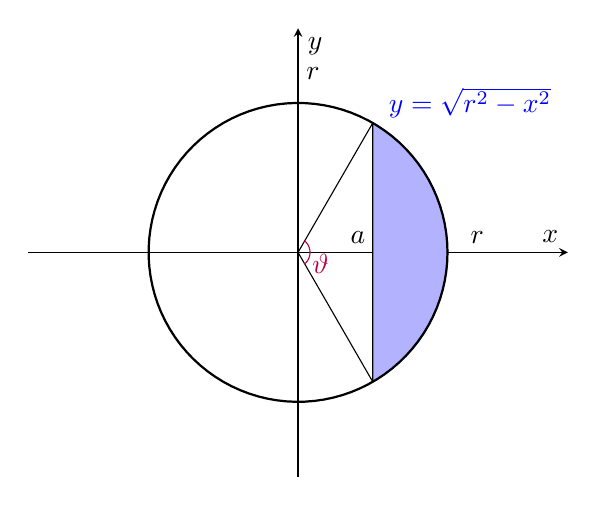
\begin{tikzpicture}

\begin{axis}[
axis equal,
xlabel=$x$, 
ylabel=$y$,
xmin = -1.5, xmax = 1.5, ymin = -1.5, ymax=1.5,
grid = none,
axis lines = center,
xtick={0},
ytick={0}
]

        
        \addplot [domain=-60:60, samples=50, fill=blue!30] ({cos(x)}, {sin(x)}) -- (axis cs:0.5,0) -- cycle;
        \addplot [domain=0:360, samples=100, thick] ({cos(x)}, {sin(x)});
        \addplot[domain=0:0.5, samples = 2]{1.732*x};
        \addplot[domain=0:0.5, samples = 2]{-1.732*x};
        \addplot [domain=-52:52, samples=100] ({cos(x)/10-0.02}, {sin(x)/10})[purple];
        \node at (axis cs:0.1,1.2) {$r$};
        \node at (axis cs:1.2,0.1) {$r$};
        \node at (axis cs:0.4, 0.1) {$a$};
        \node at (axis cs:0.15, -0.08){\textcolor{purple} {$\vartheta$}};
        \node at (axis cs:1.15,1){\textcolor{blue}{$y=\sqrt{r^2-x^2}$}};
        

\end{axis}
\end{tikzpicture} 
De oppervlakte is: $$A = 2\cdot \int_a^r \sqrt{r^2-x^2}\,dx$$
Stel $x=r\cos t$ en $t\in\left[0,\pi\right]$, dan is $dx =-r\sin t\, dt$. \\
Dan is $$\sqrt{r^2-x^2}\,dx = \sqrt{r^2-r^2\cos^2t}\, dx=r\sqrt{\sin^2t}\left(-r\sin t\right)\,dt = -r^2\sin^2t\,dt.$$

Als $x=a$, dan is $r\cos t = a$ of $t=\text{bgcos}\frac{a}{r} = \frac{\vartheta}{2}$.\\.\\
Als $x=r$, dan is $r\cos t = r$ of $t=0$.\\
Dus $$A = 2\cdot\int_a^r \sqrt{r^2-x^2}\, dx =-2r^2\int_\frac{\vartheta}{2}^0\sin^2t\,dt = -2r^2\int_\frac{\vartheta}{2}^0 \frac{1-\cos2t}{2}\,dt = -r^2\left[t - \frac{\sin2t}{2}\right]_\frac{\vartheta}{2}^0$$ $$=-r^2\left(-\frac{\vartheta}{2}+\frac{\sin\vartheta}{2}\right) = \frac{r^2}{2}\left(\vartheta-\sin\vartheta\right).$$
\end{proof}
\section{Oppervlakte van een cirkelsector p.122}
\begin{Stelling}
    De oppervlakte van een cirkelsector met straal $r$ en middelpuntshoek $\vartheta$ is $\frac{r^2\vartheta}{2}.$
\end{Stelling}
\begin{proof}
    Met een hoek van $2\pi$ is de oppervlakte de hele cirkel dus $\pi r^2$. Dan is de oppervlakte van de cirkelsector met hoek $\vartheta$ gelijk aan $\pi r^2\cdot\frac{\vartheta}{2\pi} = \frac{r^2\vartheta}{2}.$
\end{proof}
\section{Volume omwentelingslichamen p.134}
Stel dat $f$ een continue functie is in $\left[a,b\right]$. We zoeken het volume $V$ van het omwentelingslichaam van $f$ tussen $a$ en $b$.
\begin{enumerate}
    \item Verdeel $\left[a,b\right]$ in $n$ intervallen met breedte $\Delta x = \frac{b-a}{n}.$
    \item Kies in elk interval een willekeurige $c_i$. We bouwen een rechthoekje met breedte $\Delta x$ en hoogte $\left|f\left(c_i\right)\right|$.
    \item We wentelen dit om de x-as en krijgen een cilinder met volume\\ $\Delta x \cdot \pi \cdot\left(f\left(c_i\right)\right)^2.$
    \item De som van alle cilinders is $$V_n = \sum_{i=1}^n\Delta x \cdot \pi \cdot\left(f\left(c_i\right)\right)^2.$$
    \item De limiet hiervan is het gevraagde volume $$V = \lim_{n\to +\infty} \sum_{i=1}^n\Delta x \cdot \pi \cdot\left(f\left(c_i\right)\right)^2.$$
    \item Omdat $f$ continu is, is $\pi f^2$ ook continu. Door de definitie van bepaalde integralen is het volume gelijk aan $$V=\pi\int_a^b\left(f\left(c_i\right)\right)^2\, dx$$
\end{enumerate}
\section{Volume van een cilinder p.137}
\begin{Stelling}
    Het volume van een cilinder met hoogte $h$ en straal $r$ is $\pi r^2h.$
\end{Stelling}
\begin{proof}
   $\ll\textsc{Figuur p. 137}\gg$\\ De cilinder is gevormd door $y=r$ te wentelen om de x-as. Het volume is dus $$V = \pi\int_0^h r^2 dx= \pi r^2 \left[x\right]_0^h = \pi r^2h.$$
\end{proof}
\section{Volume van een kegel p.137}
\begin{Stelling}
    Het volume van een kegel met hoogte $h$ en straal $r$ is $\frac{1}{3}\pi r^2h.$
\end{Stelling}
\begin{proof}
   $\ll\textsc{Figuur p. 137}\gg$\\ De kegel is gevormd door $y=\frac{r}{h}x$ te wentelen om de x-as. Het volume is dus $$V = \pi\int_0^h \frac{r^2}{h^2}x^2 dx= \pi \frac{r^2}{h^2} \left[\frac{x^3}{3}\right]_0^h = \frac{1}{3}\pi r^2h.$$
\end{proof}
\section{Volume van een afgeknotte kegel p.138}
\begin{Stelling}
    Het volume van een afgeknotte kegel met hoogte $h$ en stralen $a$ en $b$ is $\frac{\pi h}{3}\cdot \left(b^2+ab+a^2\right).$
\end{Stelling}
\begin{proof}
    $\ll\textsc{Figuur p. 138}\gg$\\ De afgeknotte kegel is gevormd door de rechte door $(0,a)$ en $(h,b)$ om de x-as te wentelen. \\Deze rechte heeft als vergelijking $y-a = \frac{b-a}{h-0}\cdot(x-0) \iff y = \frac{b-a}{h}x+a$.
    Het volume is dus 
    \begin{alignat*}{3}
        V &= \pi\int_0^h\left(\frac{b-a}{h}x+a\right)^2 dx. \quad &&\text{Stel } t=\frac{b-a}{h}x+a\\
        & &&\text{Dan }dt = \frac{b-a}{h}\, dx\\
        \\&&&\text{Voor } x=0 \text{ is } t=a.&&\\
        &&&\text{Voor } x=h \text{ is } t=b.&&\\
    &=\frac{h}{b-a}\cdot\pi\int_a^b\left(\frac{b-a}{h}x+a\right)^2\frac{b-a}{h} dx\\ &= \frac{\pi h}{b-a}\int_a^bt^2 dt\\&= \frac{\pi h}{b-a} \cdot \left[\frac{t^3}{3}\right]_a^b\\&=\frac{\pi h}{b-a}\cdot\frac{b^3-a^3}{3}&&\left(\tiny b^3-a^3 = (b-a)(b^2+ab+a^2)\right)\\
    &=\frac{\pi h}{3}\cdot\left(b^2+ab+a^2\right)
    \end{alignat*}
\end{proof}
\newpage
\section{Volume van een bol p.139}
\begin{Stelling}
    Het volume van en bol met straal $r$ is $\frac{4\pi r^3}{3}$
\end{Stelling}
\begin{proof}
    $\ll\textsc{Figuur p. 139}\gg$\\ De bol is gevormd door $y=\sqrt{r^2-x^2}$ te wentelen om de x-as. Het volume is dus 
    \begin{align*}
        V &= \pi\int_{-r}^r (r^2-x^2) dx\\&= \pi\int_{-r}^r r^2 dx -\pi\int_{-r}^r x^2 dx\\&=\pi r^2\left[x\right]_{-r}^r - \pi\left[\frac{x^3}{3}\right]_{-r}^r\\&=\pi r^2\cdot 2r - \frac{2\pi r^3}{3}\\&=\frac{4\pi r^3}{3}.
    \end{align*}
\end{proof}\newpage

\end{document}

